\chapter{考察}
\label{chap:discussion}

実験結果を受けて,第六章ではより高精度な生成や発展的な問題設定に向けて考察をおこなう.

\section{本研究の貢献}
(TODO)

\section{課題}

\subsection{定性的な改善}
今回の研究では,尤度上はDSSMの映像予測を改善できたもののあまり定性的には改善が確認できず,特に小さい物体の生成や予測については未だうまく行かなかった.しかし比較用のVAEの実験から,これはそもそもデコーダー・エンコーダーが貧弱で物体一つ一つをはっきりと潜在表現として獲得できていないことが問題であった可能性がある.小さい物体の生成が上手くいかないのはモデルの表現力がそもそも弱かったことが原因であるとして,小さい物体の移動もあまりうまく捉えられていない理由はとして次の2つを考えた.
\begin{itemize}
    \item 生成結果がぼやけたままだと物体の移動などは捉えることが難しい
    \item そもそも条件付けられる行動が直接的には関与しない物体の移動は,DSSMでの学習が難しい
\end{itemize}
2が真の理由である場合,より根本的なDSSMの改善を考える必要があるが,素朴には遷移モデルの中間層を増やすことや,行動系列を生成するなどのアプローチが考えられる.また1が原因出あった場合には表現力の高いデコーダーを用意するなどするなどで改善が期待できるが,原因は今回の実験からは特定できないためこの問題の解明は今後の課題である.

\subsection{初期状態の推論}
今回は初期状態s0の推論には,経験的な手法として状態変数の事後分布モデルに初期観測とゼロベクトルを渡すことで生成される状態ベクトルを用いたが,これが最適なのかは定かではない.例えば自己回帰モデルを用いる強化学習では,初期状態の推論時に,学習に使う観測系列が始まる直前までの十分な長さの観測系列を使って,ゼロベクトルで表される仮の初期状態を十分な回数更新して(これをburn-inと呼ぶ)真の初期状態として用いることが良いとし,さらに初期状態の推論に用いる観測系列が長いほど精度が向上すると報告した研究がある(R2D2).本研究ではではロボットの実応用を想定しており,初期状態から予め十分先の将来を予想をした上で行動を開始して欲しいという目的意識があるためこのburn-inは直接適用できないが,同じ初期観測を用いてでも複数回状態ベクトルを更新することは有効である可能性があり,研究の余地がある.

\subsection{低階層の状態表現の再学習}
今回提案手法では,複数階層のDSSMモデルを学習させる際には低階層のモデルのパラメータを固定している.しかし学習を簡単にする上ではこれでよいものの,全体としての性能の向上を考えたときにモデルのパラメータを固定することが良いとは必ずしも言えない.今回低階層のモデルは低次元の状態表現で将来の観測の再構成ができるように学習するが,高階層のモデルの学習時には低階層のモデルは再構成しやすい表現を持つ必要はなく,むしろ高階層の状態表現を使った将来予測が簡単になるよう,例えば高階層の状態遷移を補助しやすくなるようなより中心的な状態表現とその遷移を獲得することが求められるはずである.したがって,学習のどこかの段階でモデルの低階層部分を,低階層の状態表現からのデコードをせずに再学習することで,より全体としての性能が高められる可能性が考えられる.

\section{展望}
\subsection{敵対的学習の導入}
本研究で扱ったDSSMでは損失関数に二乗誤差を利用しているため,画像空間上の小さな特徴量,例えば小さい物体や背景に近い色をした物体などは無視されやすい.二章で取り上げたVAEやDSSMなど最尤推定を用いる深層生成モデルは目的関数に生成誤差を取るために一般的に共通してこのような問題を持つ.この問題は,近年高品質な深層生成モデルとして研究が盛んな敵対的生成ネットワーク,GAN(generative adversarial networks)を補助的に用いることによる解決などが考えられる.

\subsection{多視点からの映像予測}
本研究では1視点からの映像予測を行っているが,ロボット実機に映像予測を応用する際にはロボットの視点が動くような問題設定や,より高性能な予測を行うために多視点からの
観測が使える前提で映像予測を行うというような問題設定なども考えられる.
深層学習研究で複数視点からの観測を扱う問題の先行研究としてGeneration Query Network(GQN)[]があり,複数視点からの観測とその視点位置が与えられたときに別の視点からの観測を予測して生成する問題を解いている.この研究では視点不変な共通の潜在変数の獲得を行い,クエリとして視点情報が渡されたときにその視点での観測を返すモデルを考えている.DSSMにGQNのアプローチを組み合わせることは,より良い表現の獲得と実用性の向上につながるため重要であり,実際Temporal GQNなどこの方向性の研究はすでに進められているが,このような問題設定においても本研究の提案手法は有効であると考えられるので検証を行いたい.

\subsection{他の構造を持つ潜在表現との併用}
今回の提案手法では潜在変数の階層性のみを仮定してモデルを構築したが,近年の映像予測モデルのほとんどは潜在変数に平面的な構造を仮定し,状態表現をベクトルではなく行列として扱うことで性能の向上を実現している[high fide, SVG].状態表現に階層性をもたせることの有効性は実験で示したとおりであるが,他にも環境内でより立体的な行動を考える際には潜在変数に立体性を仮定したり,さらに例えば操作対象の物体が1つで構造が既知の場合には操作対象のメッシュ情報やグラフ構造を状態表現の構造として用いることも可能であると考えられる.
このようなベクトル以外の構造を持つ状態表現を学習したい場合においても,低次元のベクトル状の潜在表現を用いて階層的なモデルを考えることで精度を高めたり学習をスムースに進められるようになる可能性があり,本研究の提案アルゴリズムが活かせると考える.

\subsection{メタ学習の導入}
機械学習研究において,似たタスク集合が与えられたときにそれらのタスク全てに汎化できるようなモデルの獲得を目指すメタ学習という研究分野がある.行動条件付き映像予測では与えられたデータから環境の遷移を学習するが,遷移自体が同じで観測が異なるような場合,例えば本研究で扱ったBAIR Push Datasetをベースに考えると机や操作対象の物体,そしてロボットの操作方策は同じままロボットの機種だけが異なるような場合にも適切に映像予測がしたいというような問題設定が考えられるが,このような設定ではメタ学習手法を用いることで様々なロボットに対応できる映像予測が可能になる.この場合具体的には,状態表現にロボットの機種情報が含まれないよう状態表現とロボットの機種クラスの相互情報量を最小化する制約を置いて遷移を学習することでロボットの機種に依存しない遷移モデルを獲得することができ,代わりにデコーダーにロボットの機種クラス情報を追加で渡すことで適切に映像予測が可能になると予想できる.

\subsection{映像予測用データ収集の人による代替}
映像予測を行うにはまずデータを収集する必要があるが,映像予測の実ロボットでの応用を考えた場合,BAIR Push Datasetのようにランダムにロボットを動かしてデータを集めるだけでは本来不十分である.理想的には,実ロボットが環境中である程度期待する動きをすることがわかっている場合にも,期待する行動系列をまんべんなく試行してデータを集めたい.
しかしそもそもロボットが環境を適切に操作するための制御方策を獲得すること自体難しいことが多く,適切に映像予測用のデータが集められるような良い制御方策が獲得できていればわざわざ映像を予測する必要はないかもしれない.
そこで,考えられるのがデータの収集を人間が行う方法で,人間であれば環境内で期待する様々な行動系列実行することは容易い.ここで以下の二つの問題が発生するがこれらは近年の研究や技術で簡単に解決することが見込める.
\begin{itemize}
    \item ロボットとは異なり,人間の行動系列情報を取得することが難しい
    \item データセットでは人間が,実環境ではロボットが操作を行うため,適切に映像予測を学習できても実機ロボットの映像予測に利用できない
\end{itemize}

まず一点目については,これは操作主体の人をカメラや工学センサー,磁気センサーなどを使ったモーショントラッキングやモーションキャプチャの技術によって人の行動系列(この場合人の運動)を計測することができる.二点目については,例えばTCNで提案されているような手法で,同じ操作を行う人間の行動系列データとロボットの行動系列データの対応関係を予め学習した上で,データセットとロボットの実観測から人やロボットが写り込んでいる部分を削除してこれまで通り遷移モデルを学習・利用するアプローチが考えられる.

このようにしてロボットの代わりに人がデータを集めることで,非剛体物の操作などより複雑な映像予測の問題設定を扱うことが可能になると考える.

\section{社会応用}
本研究ではDSSMの拡張を考えたが,DSSMあるいは映像予測の研究の社会応用の可能性を
述べる.
\subsection{実機ロボットへの応用}
(考え中TODO)

\subsection{物理シミュレーションの近似}

本研究で扱った深層学習ベースの行動条件付き映像予測では物理現象の結果として観測されるデータの予測を行うが,これは物理現象の近似という意味で現行の物理シミュレーションソフトウェアと共通の目的を持っていると解釈ができる.現在,物理シミュレーションの手法としては,既知の様々な物理法則を記述し微小時間・微小空間単位で逐次的に各領域の状態を計算して全体の結果を予測することが一般的である.しかしこのアプローチは,物理法則が既知である必要があり,また複雑な物理法則に対しては予測に膨大な時間がかかりリアルタイムに予測ができないという問題がある.例えば[文献]は,蕎麦にオイスターソースをかけて混ぜる物理シミュレーションを扱っているが,1フレームごとの見た目はとてもリアルなものの物理現象としては依然不自然な部分があり,さらに30fpsで1秒の予測をするのに29時間かかると報告している.現行の物理演算ベースの映像予測に対し深層学習ベースの映像予測は,物理法則の正しさや多視点から見た際の一貫性が保証できないなど機能として制限は多いものの,必ずしも物理現象が既知である必要はなく,また一度学習すればリアルタイムで予測を行うことができる.さらに,必要なデータを集めることで機能の制限を解消することもできるはずである.このようなことから,映像予測手法は複雑な物体の物理シミュレーションの機能を部分的に代替できる可能性があり,これによってシミュレートできる物体や現象の幅が広げられると考える.

\subsection{微分可能な環境モデルとしての利用}

\begin{figure}
    \begin{center}
      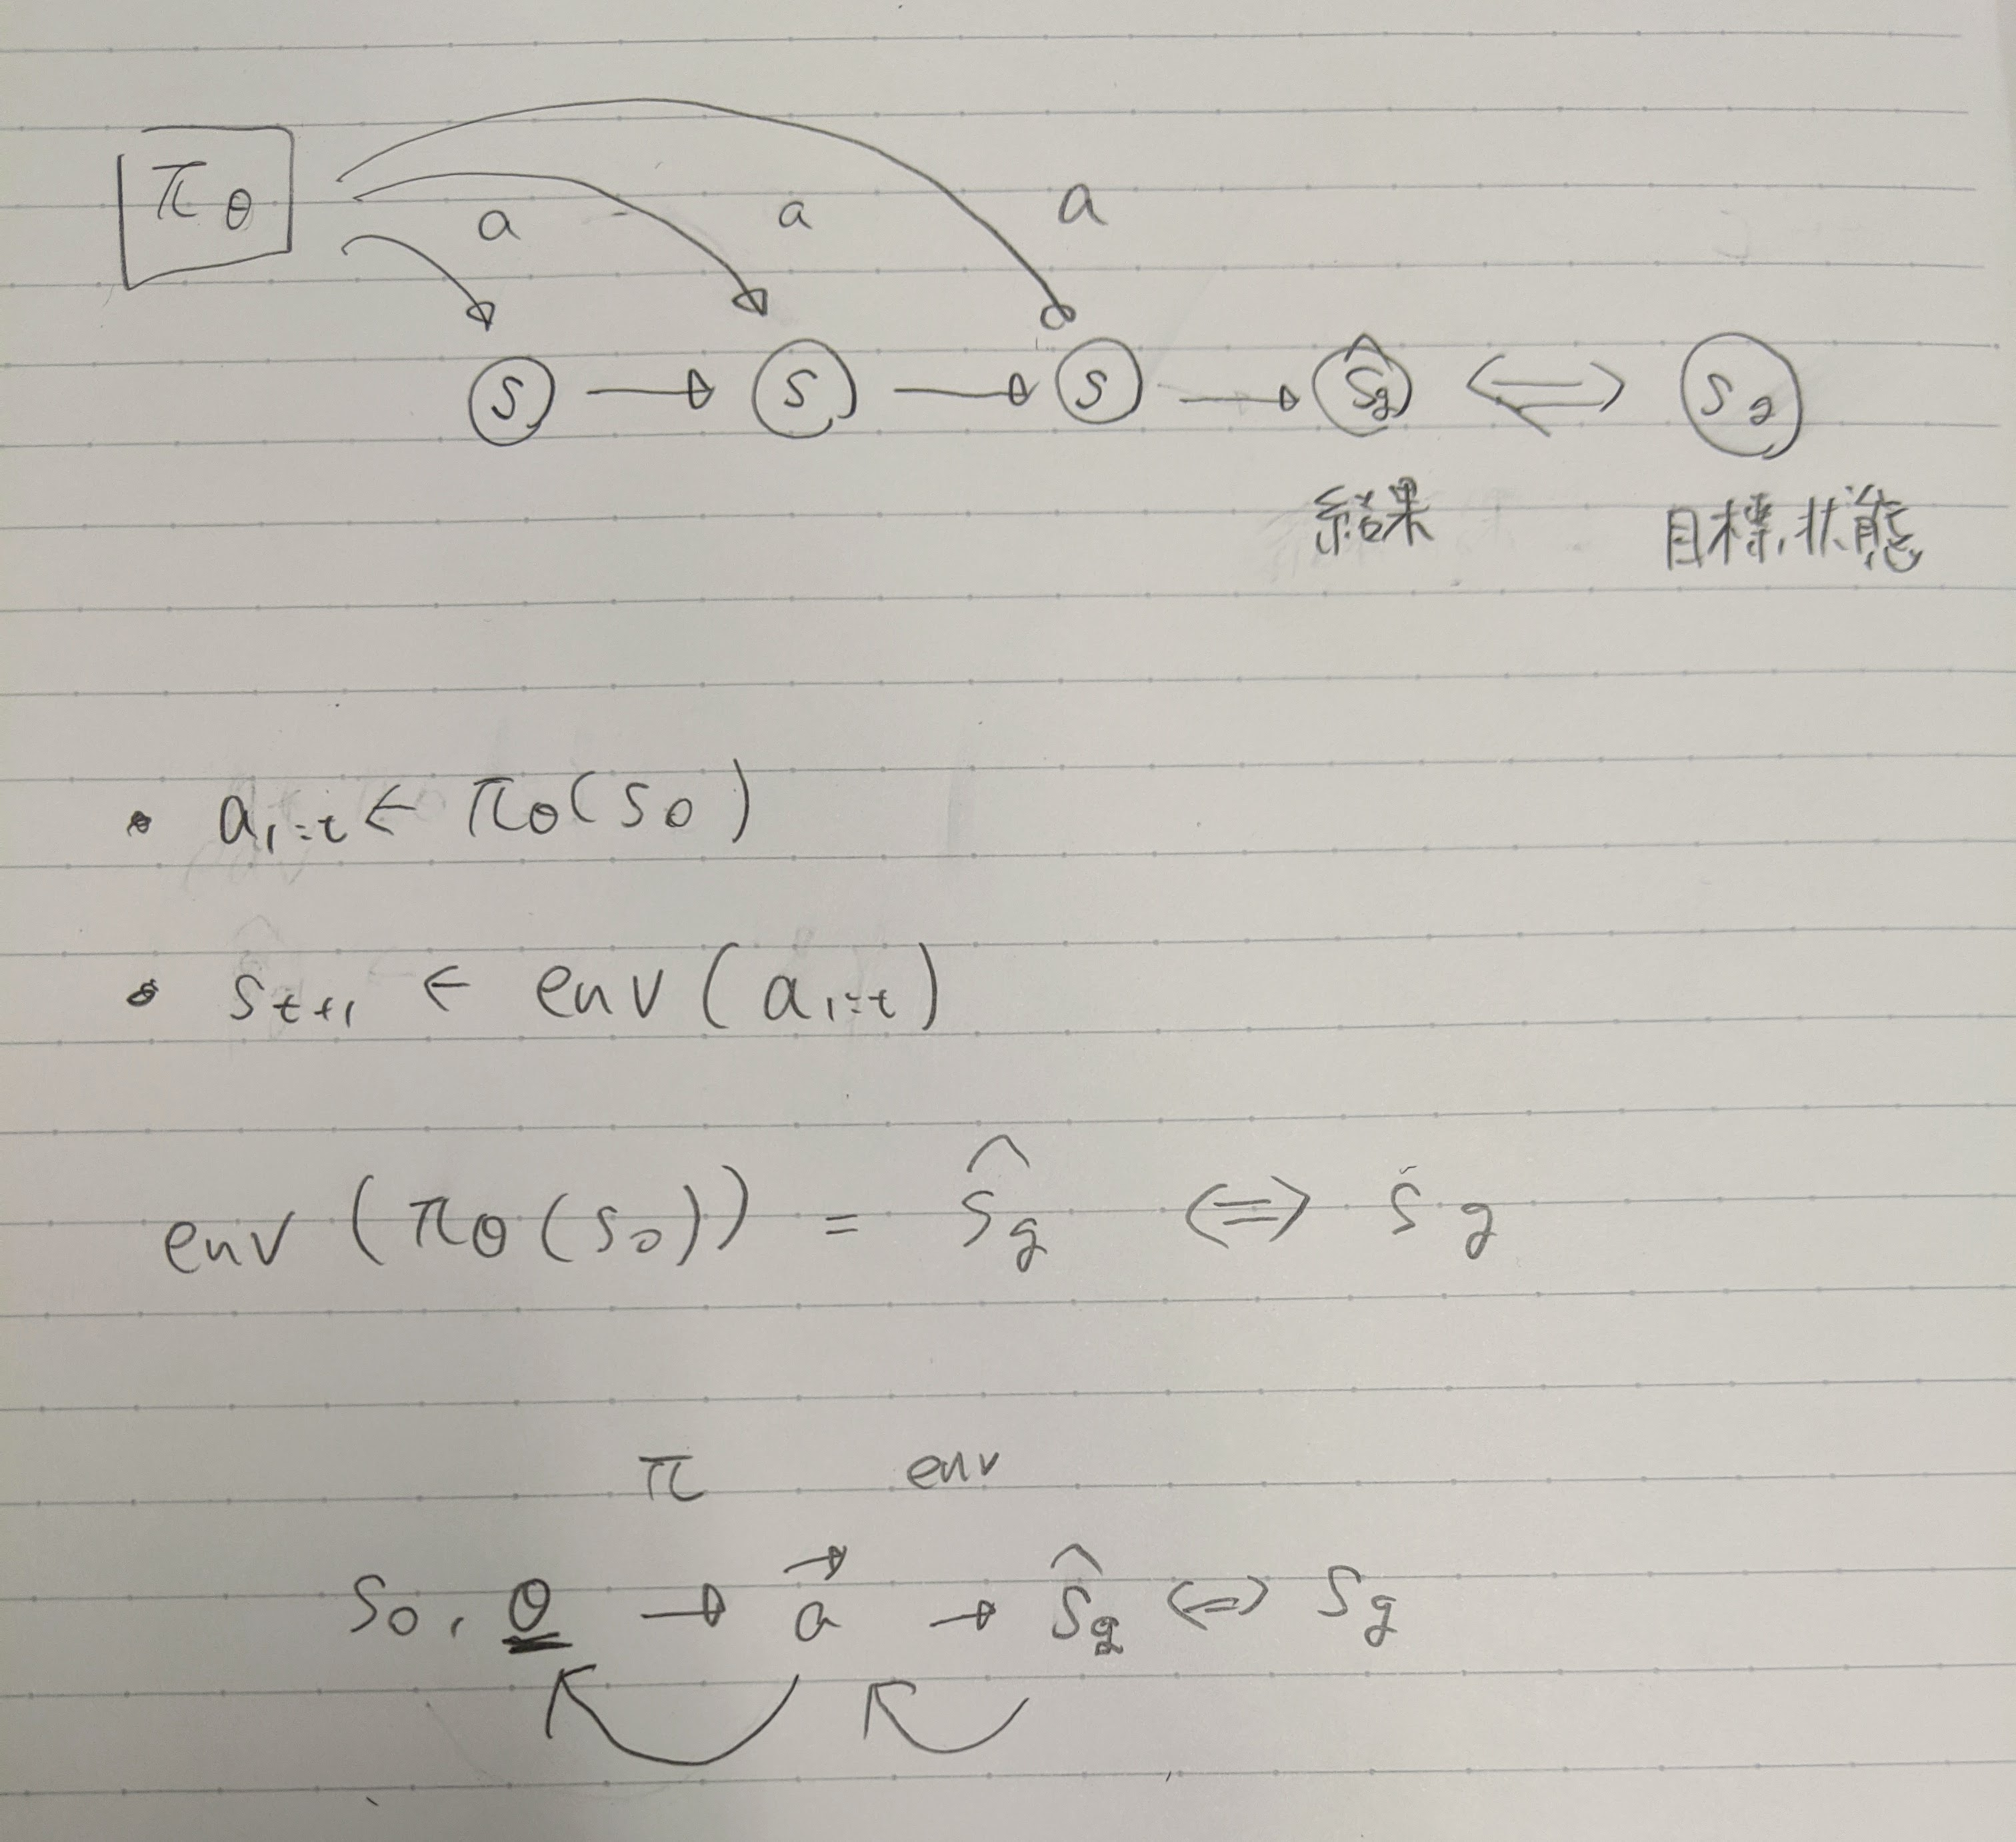
\includegraphics[width=\linewidth]{./figures/MWD.jpg}
      \caption[TODO:この図きれいにする]{TODO:きれいにする}
      \label{fig:MWD}
    \end{center}
  \end{figure}

  深層学習を用いてロボットの制御方策を学習するロボット学習において,基本的にロボットは実環境かシミュレーション環境で行動を起こすまでは結果を観測することができない.これは,ロボットの行動を入力,その結果の観測を出力と考えると,入力と出力の間に環境という未知の関数が存在し,得られた出力から入力を最適化する際に直接勾配法を用いることができないことを意味する.深層強化学習ではこの問題を様々なアプローチで解決しているが,それでも環境中で多くの試行を重ねる必要があり学習に時間がかかる上,エージェントの経験の偏りによって獲得される方策が変わってくるため性能を安定して上げることは難しい.近年の深層強化学習研究では環境との相互作用からエージェントが自ら環境のモデル自体を明示的に学習し,この学習された環境({\bf 世界モデル}/{\bf 内部モデル})を代わりに使うことで実環境での試行回数を減らし学習効率を高めるアプローチが精力的に研究されている.
  この世界モデルと同じような発想で,実機ロボットにおいて行動と結果の間に環境という未知の関数があるならば,環境という関数自体を微分可能なモデルで近似できれば,ロボットの行動方策を直接勾配法で最適化できるはずであるとする考えがある[引用].(TODO 図を入れる)具体的には,近似した環境モデル$env$と最適化したい制御方策$\pi$を用いてロボットがある初期状態$s_{start}$からある目標状態$s_{goal}$までの行動をプランニングしたときに,環境モデル$env$によって予測される結果状態$\hat{s}_{goal}$との誤差を小さくするように勾配法で直接方策を学習する.

  \begin{eqnarray}
    env(\pi(s_{start})) = \hat{s}_{goal} \Leftrightarrow s_{goal} \nonumber
  \end{eqnarray}

  ここで,本研究のようなディープラーニングベースの環境の近似モデルは微分可能であるため,この式で示す方法での方策の最適化に用いることができる.特に環境が既知で,予め他のエキスパートロボットやあるいは人間によって多くの試行を重ねてデータの収集ができ,環境を非常に高い精度で近似できる場合には,この近似モデルを使った方策の学習は非常に有効であると考えられる.このように映像予測手法が発展することによって,全く新しいアプローチのロボット学習の研究が可能になり,近似環境モデルを用いた素早く安定した学習によってロボットの応用の可能性が広がると考えている.
  
  
